\documentclass[border=10pt]{standalone}
\usepackage{tikz}\usepackage{amsmath}\usetikzlibrary{arrows.meta}
\begin{document}
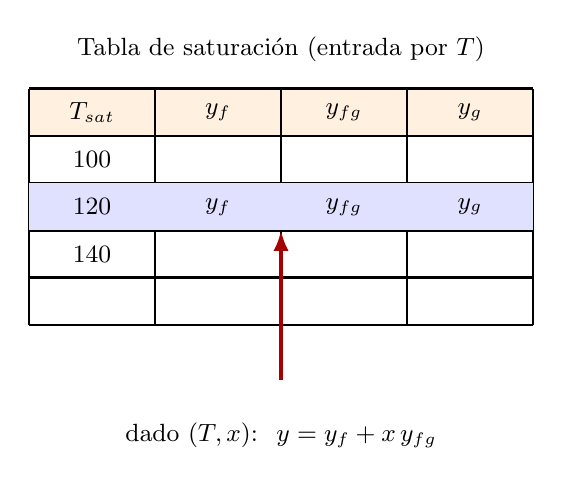
\begin{tikzpicture}[line width=1pt,>={Latex[length=2.6mm]}]
  % tabla
  \def\cols{0,1.6,3.2,4.8,6.4}
  % cabecera
  \fill[orange!12] (0,2.4) rectangle (6.4,3.0);
  \foreach \x in {0,1.6,3.2,4.8} \draw (\x,0) -- (\x,3.0);
  \draw (6.4,0)--(6.4,3.0);
  \foreach \y in {0,0.6,1.2,1.8,2.4,3.0} \draw (0,\y)--(6.4,\y);
  \node at (0.8,2.7){\small $T_{sat}$};
  \node at (2.4,2.7){\small $y_f$};
  \node at (4.0,2.7){\small $y_{fg}$};
  \node at (5.6,2.7){\small $y_g$};
  % filas (valores ilustrativos)
  \foreach \y/\t in {1.8/100,1.2/120,0.6/140} \node at (0.8,\y+0.3){\small \t};
  % fila resaltada
  \fill[blue!12] (0,1.2) rectangle (6.4,1.8);
  \node at (0.8,1.5){\small 120};
  \node at (2.4,1.5){\small $y_f$};
  \node at (4.0,1.5){\small $y_{fg}$};
  \node at (5.6,1.5){\small $y_g$};
  % flecha y formula
  \draw[->,red!65!black,line width=1.3pt] (3.2,-0.7)--(3.2,1.2);
  \node[align=center] at (3.2,-1.4){\small dado $(T,x)$:\; $y=y_f+x\,y_{fg}$};
  \node at (3.2,3.5){\small Tabla de saturación (entrada por $T$)};
\end{tikzpicture}
\end{document}
